\documentclass[svgnames]{article}
\usepackage{pgfgantt}
\usepackage{xcolor}
\usepackage{tcolorbox}
\usepackage{sectsty}
\usepackage{titlesec}
\usepackage{chronology}
\usepackage{fontawesome}
\usepackage{academicons}
\usepackage{hyperref}
\usepackage{tabularx}
\usepackage{marvosym}
\usepackage{ifsym}
\usepackage[scale=0.92]{geometry}
\usepackage{tikz}
\usepackage{colortbl}
\usetikzlibrary{calc}
\usetikzlibrary{decorations.pathmorphing}
\usetikzlibrary{arrows.meta}
\urlstyle{rm}

% Colors
\definecolor{CVblue}{HTML}{1483D3}
\definecolor{CVmain}{HTML}{6F6F6F}
\definecolor{CVsecondary}{HTML}{8ED08F}
\definecolor{CVter}{HTML}{FFE77A}

\definecolor{CVgrey}{HTML}{E6E6E6}
\sectionfont{\color{CVmain}}
\subsectionfont{\color{white}}

\newcommand*\circled[1]{\tikz[baseline=(char.base)]{
            \node[shape=circle,draw,inner sep=1pt,color=CVmain] (char) {#1};}}

% Fonts
\usepackage{fontspec}
\setmainfont{Carlito}
%\newfontfamily\thesubsectionfont{/home/ctroupin/.fonts/D-DIN.ttf}
\newfontfamily\thesubsectionfont[Path = /home/ctroupin/.fonts/,Color=CVmain]{D-DIN}
\titleformat*{\subsection}{\large\thesubsectionfont}
%\urlstyle{rm}

\hypersetup{bookmarksopen=true,
bookmarksnumbered=true,  
pdffitwindow=false, 
pdfstartview=FitH,
pdftoolbar=false,
pdfmenubar=false,
pdfwindowui=true,
pdfauthor=Charles Troupin,
pdftitle=Charles Troupin Curriculum,
pdfsubject=C. Troupin Resume,
colorlinks=true,%
breaklinks=true,%
linkcolor=CVmain,anchorcolor=CVmain,%
citecolor=CVmain,filecolor=blue,%
menucolor=CVmain,%
urlcolor=CVmain}

\newcommand{\fourstar}{\footnotesize \textcolor{CVmain}{\faStar\faStar\faStar\faStar}}
\newcommand{\threestar}{\footnotesize \textcolor{CVmain}{\faStar\faStar\faStar}\faStarO}
\newcommand{\twostar}{\footnotesize \textcolor{CVmain}{\faStar\faStar}\faStarO\faStarO}
\newcommand{\onestar}{\footnotesize \textcolor{CVmain}{\faStar}\faStarO\faStarO\faStarO}
\newcommand{\halfstar}{\footnotesize \textcolor{CVmain}{\faStarHalfO}\faStarO\faStarO\faStarO}

\newcommand{\sepa}{$\cdot$~}
\newcommand{\role}[1]{\textbf{#1}}

% Ovale box for the skills
\newtcbox{\skillbox}{nobeforeafter,colframe=CVmain,colback=white,boxrule=1pt,arc=4pt,height=0.5cm,
  boxsep=0pt,left=3pt,right=3pt,top=2.5pt,bottom=2pt,box align = center}
  

  
\titlespacing*{\subsection}{0pt}{1ex}{-0ex}
\titlespacing*{\subsubsection}{0pt}{1ex}{-0ex}

\begin{document}

\pagestyle{empty}

\begin{tikzpicture}[overlay,remember picture]
    \draw [dashed,line width=.4mm,color=CVmain]
        ($ (current page.north west) + (.25cm,-.25cm) $)
        rectangle
        ($ (current page.south east) + (-.25cm,.25cm) $);
\end{tikzpicture}

\vspace{-.7cm}

{\centering \LARGE{\thesubsectionfont Charles Troupin}} {\large \sepa Data analyst \& modeler \sepa Engineer in Physics}

\begin{tabular*}{.65\textwidth}{cl!{\color{CVmain}\vrule}cl}
\circled{\faMobile} & +32~498~155~998 \hspace{5cm} & \circled{\faSkype} & charles.troupin1 	 \\
\circled{\faEnvelope} & \href{mailto:ctroupin@protonmail.com}{ctroupin@protonmail.com} & \circled{\faHome}	& \url{http://ctroupin.github.io}\\
\circled{
\includegraphics[height=1.6ex]{gitlab_logo_grey.png}} & \url{https://gitlab.com/ctroupin} & \circled{\faGithubSquare} & \url{https://github.com/ctroupin/} \\
\circled{\aiOrcidSquare} & \url{http://orcid.org/0000-0002-0265-1021} & \circled{\faTwitterSquare} &  \url{https://twitter.com/CharlesTroupin} \\
\end{tabular*}

\subsection*{Professional experience}

\begin{tikzpicture}

    \node[anchor=south west,inner sep=0cm] (image) at (0,0) {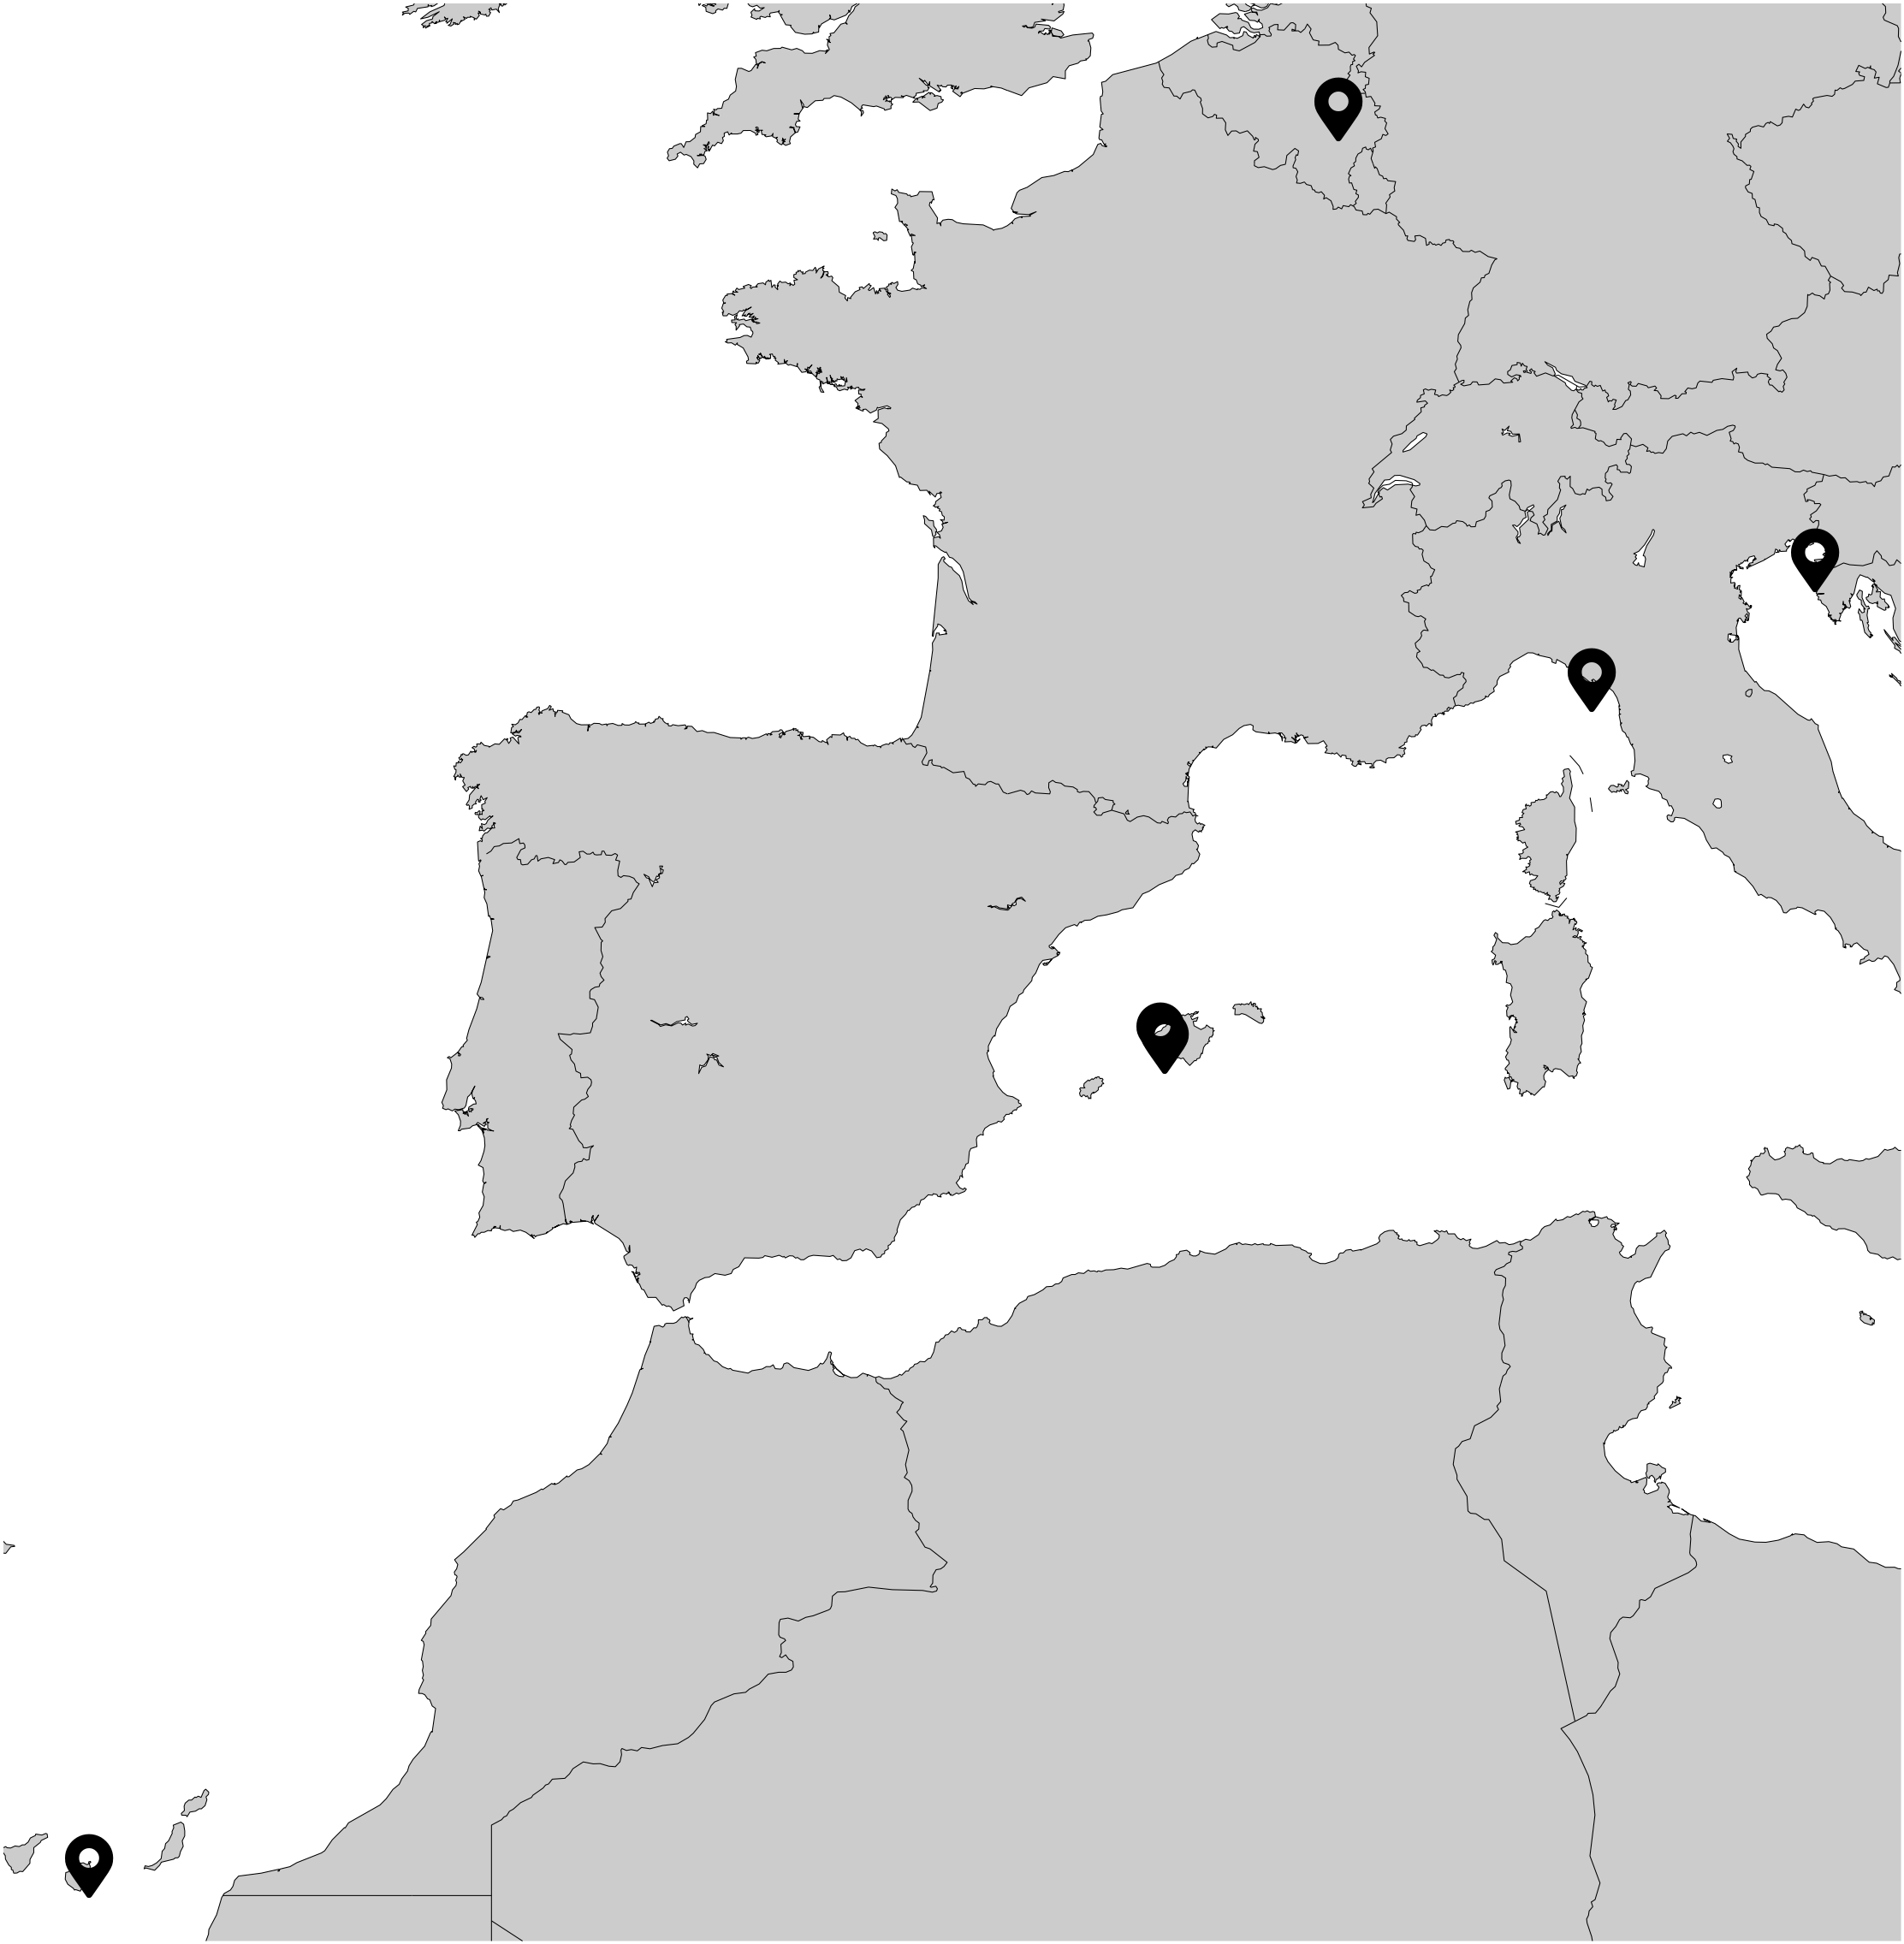
\includegraphics[width=.3\textwidth]{./figures/employment_map.png}};
    \begin{scope}[x={(image.south east)},y={(image.north west)}]
%    \draw[help lines,xstep=.1,ystep=.1] (0,0) grid (1,1);
%    \foreach \x in {0,1,...,9} { \node [anchor=north] at (\x/10,0) {0.\x}; }
%    \foreach \y in {0,1,...,9} { \node [anchor=east] at (0,\y/10) {0.\y}; }
    \node [anchor=west,text width=.65\textwidth,minimum height=1cm] (n2017) at (1.1,.95){2017/01--present\dotfill \textbf{Post-doctoral researcher \faAt~\href{http://labos.ulg.ac.be/gher/}{GHER} (ULiège)}\\ \textit{Data interpolation, visualisation and cloud computing}};
    \node [anchor=west,text width=.65\textwidth,minimum height=1cm] (n2014) at (1.1,0.75){2014/03--2017/01\dotfill \textbf{Head of the Data Centre Facility \faAt~\href{www.socib.es}{\mbox{SOCIB}}}\\ \textit{Acquisition, processing and visualisation of oceanographic and meteorological data}};
    \node [anchor=west,text width=.65\textwidth,minimum height=1cm] (n2013) at (1.1,0.55){2013/03--2014/03\dotfill \textbf{Post-doctoral researcher \faAt~\href{http://imedea.uib-csic.es/}{IMEDEA}}\\ \textit{Analysis of in situ, satellite altimetry and high-frequency radar data}};
    \node [anchor=west,text width=.65\textwidth,minimum height=1cm] (n2010) at (1.1,0.35){2010/10--2013/02\dotfill \textbf{Research assistant \faAt~\href{www.ulg.ac.be}{ULiège}}\\ \textit{Multivariate reconstruction of incomplete satellite images in the North Sea}};
    \node [anchor=west,text width=.65\textwidth,minimum height=1cm] (n2006) at (1.1,0.15){2006/10--2010/09 \dotfill \textbf{PhD Candidate \faAt~FRIA-FNRS}\\ \textit{Study of the Cape Ghir filament using numerical modeling and data interpolation}};
    
    \node [anchor=west,text width=.65\textwidth,minimum height=1cm] (publi) at (1.1,0.0){\textbf{Publication list:} \faFilePdfO
~\url{https://ctroupin.github.io/CV/publicationList.pdf}};
    
   	\node (liege) at (0.7,0.95) {};
   	\node (ulpgc) at (0.05,0.05) {};
   	\node (nurc) at (.83, .66) {};
   	\node (socib) at (.61, .46) {};
   	\node (imedea) at (.61, .46) {};
   	\node (nib) at (.95, .72) {};

    \draw [{Circle[]}-,line width=1pt, CVmain, anchor=south] (n2017) to [out=180, in=0] (liege);
    \draw [{Circle[]}-,line width=1pt, CVmain, anchor=south] (n2017) to [out=180, in=90] (nib);
    \draw [{Circle[]}-,line width=1pt, CVmain, anchor=south] (n2014) to [out=180, in=60] (socib);
    \draw [{Circle[]}-,line width=1pt, CVmain, anchor=south] (n2013) to [out=180, in=0] (imedea);
    \draw [{Circle[]}-,line width=1pt, CVmain, anchor=south] (n2010) to [out=180, in=-45] (liege);
    \draw [{Circle[]}-,line width=1pt, CVmain, anchor=south] (n2006) to [out=180, in=-90] (liege);
    \draw [{Circle[]}-,line width=1pt, CVmain, anchor=south] (n2006) to [out=180, in=0] (ulpgc);
    \draw [{Circle[]}-,line width=1pt, CVmain, anchor=south] (n2006) to [out=180, in=-15] (nurc);
    \end{scope}
\end{tikzpicture}

\subsection*{Education}
\vspace*{-.75cm}

\parbox{.52\textwidth}{
\begin{chronology}[2]{2000}{2012}{.5\textwidth}[\textwidth]
\event[\decimaldate{15}{9}{2000}]{\decimaldate{30}{6}{2005}}{\parbox{2.5cm}{\large Engineer\\ in Physics}}
\event[\decimaldate{1}{9}{2005}]{\decimaldate{15}{9}{2006}}{\parbox{2.5cm}{\large D.E.A. in\\ Oceanography\\ (modelling)}}
\event[\decimaldate{1}{10}{2006}]{\decimaldate{15}{9}{2011}}{\parbox{3cm}{\large PhD in Sciences\\ (Oceanography)}}
\end{chronology}
}\parbox{.15\textwidth}{
~\\
Engineering\\
Fluid mechanics\\
Aerodynamics
}\parbox{.24\textwidth}{
~\\
Finite-element method\\
Numerical simulations\\
High-performance computing
}

\subsection*{Technical skills}
\vspace*{-.5cm}

\parbox{.24\textwidth}{
\textbf{Programming}\\
Functional programming 						\\ 
Object oriented programming				\\
Test-oriented development					\\
Control version system (git, svn)			\\
Jupyter-notebooks							\\
Continuous integration\\	
%Data formats (json, csv, gpx, shapefiles)\\
}\parbox{.72\textwidth}{
\ganttset{bar height=.3}
\begin{ganttchart}[
	canvas/.style={fill=white},
    hgrid style/.style={draw=black!5, line width=.75pt},
    vgrid={*1{draw=CVmain, line width=.75pt, dashed},*2{draw=CVsecondary, line width=.75pt, dashed}},
    title/.style={draw=none, fill=none},
    title label font=\bfseries,
    title label node/.append style={below=7pt},
    include title in canvas=false,
    bar label font=\mdseries\small\color{black!70},
    bar label node/.append style={left=.2cm},
    bar/.append style={draw=none, fill=black!63},
    bar incomplete/.append style={fill=black!70},
    bar progress label font=\mdseries\footnotesize\color{black!70},
    bar progress label node /.style=east,
    y unit chart=.5cm,
    progress=today,
    today=1,
    today label={}, 
    today rule /.style={draw=CVmain, line width=.75pt, dashed},
    progress label text = ,
    ]{1}{14}
   \gantttitle[title label node/.append style={below left=5pt and -3pt}]{Languages\quad}{0}
  %\gantttitle[title/.style={draw=CVmain,below=7pt}]{Languages}{0}
  \gantttitlelist[title/.style={draw=none, inner color=CVgrey,below=7pt}]{2006,2009,...,2020}{3} \\
  \ganttbar[name=bash, progress label text={awk, makefiles, cron, git, ssh, regex, \ldots}]{Bash}{1}{16} \\
  \ganttbar[name=fortran,progress label text={data I/O, format conversion, optimisation}]{Fortran}{1}{15} \\
  \ganttbar[name=matlab,progress label text={\hspace{4cm}geostatistics, plotting, neural networks}]{MATLAB}{1}{8} \\
  \ganttbar[name=python,progress label text={matplotlib, numpy, scipy, pandas, virtualenv, \ldots}]{Python}{8}{16} \\
  \ganttbar[name=julia,progress label text={DataArrays, PyPlot, module developments}]{Julia}{11}{16} \\
  \ganttbar[name=javascript,progress label text={Leaflet, Highcharts, D3, Angular, Reveal}]{Javascript}{11}{16}
\end{ganttchart}
}

\noindent \textbf{Data analytics} 

\noindent \skillbox{Geostatistics} \skillbox{Big data} \skillbox{Predictive modelling} \skillbox{Cloud computing} \skillbox{Data visualisation}\\ 
\skillbox{Neural networks} \skillbox{Signal processing} \skillbox{Open data} 
\vspace{2mm}

%\noindent \textbf{Web} HTML, CSS, markdown, javascript, Bootstrap, Jekyll, wordpress, Dokuwiki, Mediawiki

\noindent \textbf{Oceanography} 

\noindent \skillbox{Numerical modelling (ROMS)} \skillbox{Spatial interpolation} \skillbox{Remote-sensing data reconstruction} \skillbox{Quality control} \skillbox{Eddy-tracking} \skillbox{Glider data} \skillbox{High-frequency radar data} \skillbox{Air-sea interactions} \skillbox{Small scale processes}

\subsection*{Soft skills}
\textbf{Project management:} Planning and monitoring \sepa scientific and technical reporting \sepa specification documents and strategic plans \sepa team leading, recruitment \sepa applications for grants and supports \sepa lean and agile management\\
\textbf{Communication:} Presentations at international conferences (English, Spanish, French) $\cdot$~ design of posters and leaflets (Darktable, GIMP, ImageMagick, Inkscape) $\cdot$~ social networks \sepa scientific outreach\\ 
\textbf{Organisation:} International scientific meetings (~200 participants from 40 countries) $\cdot$~ User training workshops\\
\begin{tabularx}{\textwidth}{@{}lrlr @{}}
\textbf{Languages }	& \dotfill	 	& French (native)		& \fourstar \\ 
English 			& \threestar  	& Spanish				& \threestar\\	
Catalan 			& \twostar		& Italian				& \onestar	\\
German				& \onestar		& Dutch 				& \halfstar	\\			
\end{tabularx}


\subsubsection*{Personal interests}
%---------------------------
\begin{tabular}{rlrlrlrl}
\textcolor{CVmain}{\faCameraRetro}	& Photography 				& \textcolor{CVmain}{\faMapSigns} 	& Ultra-trail and mountain running	& \textcolor{CVmain}{\faMapMarker} 	& Maps 						& \faWordpress	&Travel blogging 		\\ 		
\textcolor{CVmain}{\Bicycle}		& Road cycling& \textcolor{CVmain}{\faCloud} 	& Weather observation \& forecast		& \textcolor{CVmain}{\Industry}    	& UrbEx 	& 			& Coaching  			\\
\end{tabular}
\textcolor{white}{Last modified: \today}

%\begin{tcolorbox}[title=\subsubsection*{Personal interests},width=.5\textwidth,arc=0mm]
%\begin{tabular}{rl|rl}
%\faCameraRetro	& Photography 				& \faMapSigns 	& Ultra-trail and mountain running	\\ 		
%\faMapMarker 	& Maps 						& \faWordpress	&Travel blogging 					\\
%\Bicycle		& Road cycling& \faCloud 	& Weather observation \& forecast					\\
%\Industry    	& UrbEx 					& 							& Coaching  			\\
%\end{tabular}
%\end{tcolorbox}


	

\end{document}
